\documentclass[11pt,a4paper]{article}
\usepackage[T1]{fontenc}
\usepackage[utf8]{inputenc}
\usepackage{lmodern,microtype,amsmath,amssymb,amsthm,mathtools}
\usepackage[margin=27mm]{geometry}
\usepackage{graphicx,booktabs,array,enumitem,xcolor}
\usepackage{hyperref}
\usepackage{fancyhdr}
\definecolor{ink}{HTML}{45315D}
\hypersetup{colorlinks=true,linkcolor=ink,citecolor=ink,urlcolor=ink,
 pdftitle={Signed Kuramoto networks inside positive ones},pdfauthor={Anonymous}}
\pagestyle{fancy}\fancyhf{}
\fancyhead[L]{\small Signed Kuramoto networks inside positive ones}
\fancyhead[R]{\small v1.0.0-candidate, doi:10.5281/zenodo.23690073}
\fancyfoot[C]{\thepage}
\setlength{\headheight}{14pt}
\setlength{\parskip}{3pt}
\setlist{itemsep=2pt,topsep=4pt}
\newtheorem{theorem}{Theorem}
\newtheorem{lemma}[theorem]{Lemma}
\newtheorem{corollary}[theorem]{Corollary}
\newtheorem{proposition}[theorem]{Proposition}
\theoremstyle{definition}\newtheorem{conjecture}{Conjecture}
\theoremstyle{remark}\newtheorem{remark}[theorem]{Remark}
\newcommand{\T}{\mathbb T}
\newcommand{\R}{\mathbb R}
\newcommand{\Z}{\mathbb Z}
\newcommand{\ii}{\mathrm{i}}
\newcommand{\E}{\mathcal E}
\newcommand{\Sset}{\mathcal S}
\DeclareMathOperator{\im}{Im}
\DeclareMathOperator{\rank}{rank}
\DeclareMathOperator{\interior}{int}
\title{\textbf{Signed Kuramoto networks inside positive ones}\\[5pt]
\large An exact realisation theorem, stable non-manifold equilibria,\\ and Sclosa's closed-manifold conjecture}
\author{Anonymous}
\date{27 October 2026\\[3pt]\small Unrefereed candidate, version 1.0.0-candidate. DOI: \href{https://doi.org/10.5281/zenodo.23690073}{10.5281/zenodo.23690073}}
\begin{document}
\maketitle
\vspace{-14pt}
\begin{abstract}
Networks of identical phase oscillators with attractive (positive) coupling are the simplest models of synchronisation, yet their equilibria can form whole continua whose shape decides how linearised stability tests, equilibrium counts and numerical solvers behave. We show that anything a network with mixed positive and negative couplings can do near an equilibrium, some network with only positive unit couplings also does. Concretely, every $\pm1$ signed Kuramoto network is reproduced exactly on an invariant torus of a positive unweighted network. The complete set of nearby equilibria, the Morse index, the nullity and Lyapunov stability are all preserved. We give three applications. First, a 324-vertex positive graph has a continuum of Lyapunov-stable equilibria that is not a manifold at one point: near that point it is a cone over a torus. More generally, for every $k\ge1$ there are positive graphs with stable cones over $S^k\times S^k$. Second, a 120-vertex graph has a stable equilibrium set made of crossing tori. Third, a family of graphs has stable smooth continua of every dimension. The cone example also settles the closed-manifold form of a conjecture of Sclosa. Neither the equilibrium set nor its stable part can be written as a countable union of closed manifolds, even when the pieces are allowed to be immersed. All phenomena here occur at exact symmetric resonances and are not robust to generic perturbation of the weights.
\end{abstract}

\section{Introduction}\label{sec:intro}

Let $G$ be a finite simple graph. The homogeneous Kuramoto system on $G$ is
\begin{equation}\label{eq:flow}
 \dot\theta_u=\sum_{v\sim u}\sin(\theta_v-\theta_u),\qquad \theta\in\T^{V(G)},\quad \T=\R/2\pi\Z,
\end{equation}
the negative gradient flow of
\begin{equation}\label{eq:energy}
 E_G(\theta)=\sum_{\{u,v\}\in E(G)}[1-\cos(\theta_v-\theta_u)].
\end{equation}
Every coupling is $+1$ (attractive) and all intrinsic frequencies are equal. ``Stable'' always means Lyapunov stable for an individual equilibrium. This allows neighbouring equilibria and is weaker than asymptotic stability.

\paragraph{The picture.} Think of each oscillator as a unit arrow in the plane. On the complete graph $K_n$ the force on arrow $u$ is the component of the total $Z=\sum_v e^{\ii\theta_v}$ perpendicular to it. An equilibrium is therefore either \emph{aligned}, with all arrows on one line, or \emph{balanced}, with $Z=0$, so that the arrows close up head to tail into an equilateral polygon (Figure~\ref{fig:construction}c). For odd $n$ the balanced polygons form a smooth manifold. For $n=6$ there is a special balanced state: three arrows point east and three point west. It is both aligned and balanced, and the balanced polygons near it form a cone. A punctured neighbourhood of the tip is a cylinder over the torus $S^1\times S^1$. That neighbourhood is one connected piece, and this is what makes the point hard to cut into tidy pieces. Two crossing circles also have a singular point, but their punctured neighbourhood falls into four arcs, so the crossing is harmless.

\paragraph{Why a stable singularity is surprising.} On $K_6$ the cone point is a maximum of $|Z|^2$. It is therefore unstable for the attractive flow: the arrows prefer to synchronise. One might hope that singular continua are always unstable, so that the states a physical network actually settles into are tidy. They need not be. If the sign of every coupling on $K_6$ is reversed, the balanced polygons become global energy minima and the cone becomes stable. The point of this paper is that negative couplings can be simulated exactly with positive ones. A repulsive edge is replaced by a positive matching between copies of the two oscillators whose phases differ by $\pi$. A Kuramoto network with positive unit couplings then carries a stable equilibrium continuum that is not a manifold at one point.

\paragraph{A caveat about scope.} Every phenomenon below sits at an exact resonance: unit weights, an exact equal split of the arrows, and an exactly symmetric graph. Generic changes to the weights or frequencies destroy the singularity, and nothing here is a statement about heterogeneous networks such as power grids (Section~\ref{sec:scope}).

\subsection{Main results}

A \emph{signed} simple graph $H$ carries a symmetric sign $\sigma_{ij}\in\{-1,1\}$ on each edge, with dynamics
\begin{equation}\label{eq:signed}
 \dot\phi_i=\sum_{j\sim i}\sigma_{ij}\sin(\phi_j-\phi_i)=-\partial_iE_H^\sigma(\phi),\qquad
 E_H^\sigma(\phi)=\sum_{\{i,j\}\in E(H)}\sigma_{ij}[1-\cos(\phi_j-\phi_i)].
\end{equation}
The main result is the following realisation theorem. We have not found a previous theorem that combines arbitrary $\pm1$ realisation by positive unit couplings with a uniform normal spectral gap and the transfer of complete equilibrium germs and nonlinear Lyapunov stability; the invariance step on its own is of a known type (Section~\ref{sec:prior}). The construction (Figure~\ref{fig:construction}) replaces each base vertex by a ring of six groups of $r$ clones, at phase offsets $a\pi/3$. Each positive base edge becomes a matching between groups with equal offsets. Each negative base edge becomes a matching between groups whose offsets differ by $\pi$.

\begin{theorem}[Exact realisation of signed networks]\label{thm:realisation}
Let $H$ be a signed simple graph with $n$ vertices and maximum degree $\Delta$, and let $r>4\Delta$ be an integer. The positive simple unweighted graph $G=G(H,r)$ of Section~\ref{sec:realisation} has $6nr$ vertices and $6nr^2+6r|E(H)|$ edges, and each vertex above $i$ has degree $2r+\deg_H(i)$. It contains an embedded invariant torus $F(\T^n)$ on which~\eqref{eq:flow} is exactly~\eqref{eq:signed}. For every equilibrium $\phi^\star$ of~\eqref{eq:signed}:
\begin{enumerate}[label=(\alph*)]
\item $F$ maps the germ at $\phi^\star$ of the equilibrium set of $H$ onto the germ at $F(\phi^\star)$ of the equilibrium set of $G$;
\item $F(\phi^\star)$ is Lyapunov stable if and only if $\phi^\star$ is, and $F$ also identifies the germs of the sets of Lyapunov-stable equilibria;
\item the spectrum of the Jacobian at $F(\phi^\star)$ is the spectrum at $\phi^\star$ together with eigenvalues $\le-(r/2-2\Delta)<0$. In particular the Morse index and the nullity are preserved (Corollary~\ref{cor:spectral}).
\end{enumerate}
If $H$ is connected, so is $G$.
\end{theorem}

The first application is a positive unweighted network with a stable equilibrium continuum that is not a manifold. Here $C(L)$ denotes the open cone $[0,1)\times L/(\{0\}\times L)$, and the factor $\R$ is the common-phase direction.

\begin{theorem}[A stable non-manifold continuum]\label{thm:stable}
There is a connected, simple, unweighted, $23$-regular graph $G_{6,9}$ with $324$ vertices and $3726$ edges, and an equilibrium $\theta^\star$, such that the germ of the full equilibrium set at $\theta^\star$ is
\begin{equation}\label{eq:stablecone}
 (\E_{G},\theta^\star)\cong(\R\times C(S^1\times S^1),0),
\end{equation}
and every equilibrium near $\theta^\star$ is Lyapunov stable. Neither $\E_G$ nor its set $\Sset_G$ of stable equilibria is a countable union of closed embedded topological manifolds without boundary, and neither is a countable union of immersed compact manifolds without boundary.
\end{theorem}

Further applications (Section~\ref{sec:applications}) give a 120-vertex positive graph whose stable equilibria include crossing tori; stable smooth continua of dimension $m-2$ for every odd $m$; and stable cones $\R\times C(S^{k}\times S^{k})$ for every $k\ge1$, from $G_{2k+4,r}$. Each is certified at explicit points by computation.

\subsection{Sclosa's conjecture: which reading is refuted}

Sclosa's Conjecture~1.3 has two published wordings. The arXiv version 1 (arXiv:2207.08182v1, 17 July 2022) reads:
\begin{quote}
``Conjecture 1.3. For every graph the set of equilibria of (1) is a finite union of manifolds.''
\end{quote}
The version of record~\cite{sclosa23} (SIAM J.\ Appl.\ Dyn.\ Syst.\ 22(4), p.~3269) reads:
\begin{quote}
``Conjecture 1.3. For every graph the set of equilibria of (1.1) is a finite union of closed manifolds.''
\end{quote}
In both, ``(1)'' or ``(1.1)'' is the system~\eqref{eq:flow}. Both quotations were checked against the source text of each version. Table~\ref{tab:readings} lists the natural readings and our verdict on each. A closed subset of the compact torus is compact, so ``closed'' here means compact and without boundary.

\begin{table}[h]\centering\small
\caption{Readings of Conjecture~1.3 and their status. The refuted readings fail already for $K_6$.}\label{tab:readings}
\begin{tabular}{p{7.7cm}p{6.3cm}}\toprule
Pieces allowed & Status\\\midrule
Closed (compact, boundaryless) embedded manifolds; finite or countable union. The published wording. & \textbf{False} for $K_n$, $n\ge6$ even (Theorem~\ref{thm:classification}).\\
Images of immersions of compact boundaryless manifolds; countable union. The ``branched'' reading suggested by Sclosa's remarks on $B_4$. & \textbf{False}, same graphs (Lemma~\ref{lem:immersed}).\\
Pieces closed only relative to the equilibrium set, or to the stable set. & \textbf{False} (Lemma~\ref{lem:cover}).\\
Manifolds that need not be closed (locally closed smooth submanifolds). The literal arXiv~v1 wording. & \textbf{True} for every graph, by stratification of real algebraic sets~\cite{bcr}.\\
Compact manifolds with boundary or corners. & \textbf{True} for every graph, by triangulation of compact semialgebraic sets~\cite{bcr}: closed simplices suffice.\\\bottomrule
\end{tabular}
\end{table}

The literal arXiv~v1 reading is true. In the coordinates $(\cos\theta_u,\sin\theta_u)$ the equilibrium set is a compact real algebraic set, and every such set is a finite disjoint union of smooth submanifolds, its strata~\cite{bcr}. What fails is the stronger statement that the pieces can be taken closed, which is the published wording. It fails even for immersed pieces, which is how the three intersecting tori of $B_4$ in Sclosa's own discussion are naturally described. Sclosa also writes there that the balanced set ``is a branched manifold''. Our result shows that for even $n\ge6$ this branching cannot be resolved into closed sheets, immersed or embedded.

\begin{theorem}[Complete-graph classification]\label{thm:classification}
Let $\E_n$ be the equilibrium set of~\eqref{eq:flow} on $K_n$, $n\ge1$. The following are equivalent:
\begin{enumerate}[label=(\roman*)]
\item $\E_n$ is a finite union of closed embedded smooth manifolds without boundary;
\item $\E_n$ is a countable union of closed embedded topological manifolds without boundary;
\item $\E_n$ is a countable union of images of immersions of compact topological manifolds without boundary;
\item $n$ is odd or $n\le4$.
\end{enumerate}
\end{theorem}

The local cone at the balanced aligned point of $K_{2m}$ is classical polygon-space geometry~\cite{kamiyama,kapovichmillson}. Burns et al.~\cite{burns} (arXiv:2605.22983v3, Section~16, Theorem~16.1) identify its space of tangent directions as $S^{m-2}\times S^{m-2}$ for the Kuramoto potential directly. Theorem~\ref{thm:classification} builds on that description. We give a self-contained derivation of the local homeomorphism in Kuramoto angle coordinates (Lemma~\ref{lem:cone}); an equivalent local normal form may already exist in the polygon-space literature, and we do not claim it as new. What we add is the closed- and immersed-cover obstructions (Lemmas~\ref{lem:cover} and~\ref{lem:immersed}), and the cases $n\le4$. Theorem~\ref{thm:classification} is therefore a short corollary of known geometry together with a point-set argument; its interest lies in settling the conjecture precisely.

\paragraph{Roadmap.} Section~\ref{sec:realisation} builds $G(H,r)$ and proves Theorem~\ref{thm:realisation}, including the energy inequality behind the stability transfer. Section~\ref{sec:topology} derives the local cone and the two cover obstructions. Section~\ref{sec:applications} specialises the realisation to repulsive complete graphs, proving Theorem~\ref{thm:stable} and the further applications. Section~\ref{sec:classification} proves Theorem~\ref{thm:classification}. Section~\ref{sec:verification} describes the computations, and Section~\ref{sec:prior} compares with prior work, including a priority check against coupled-cell network theory.

\begin{figure}[!htb]\centering
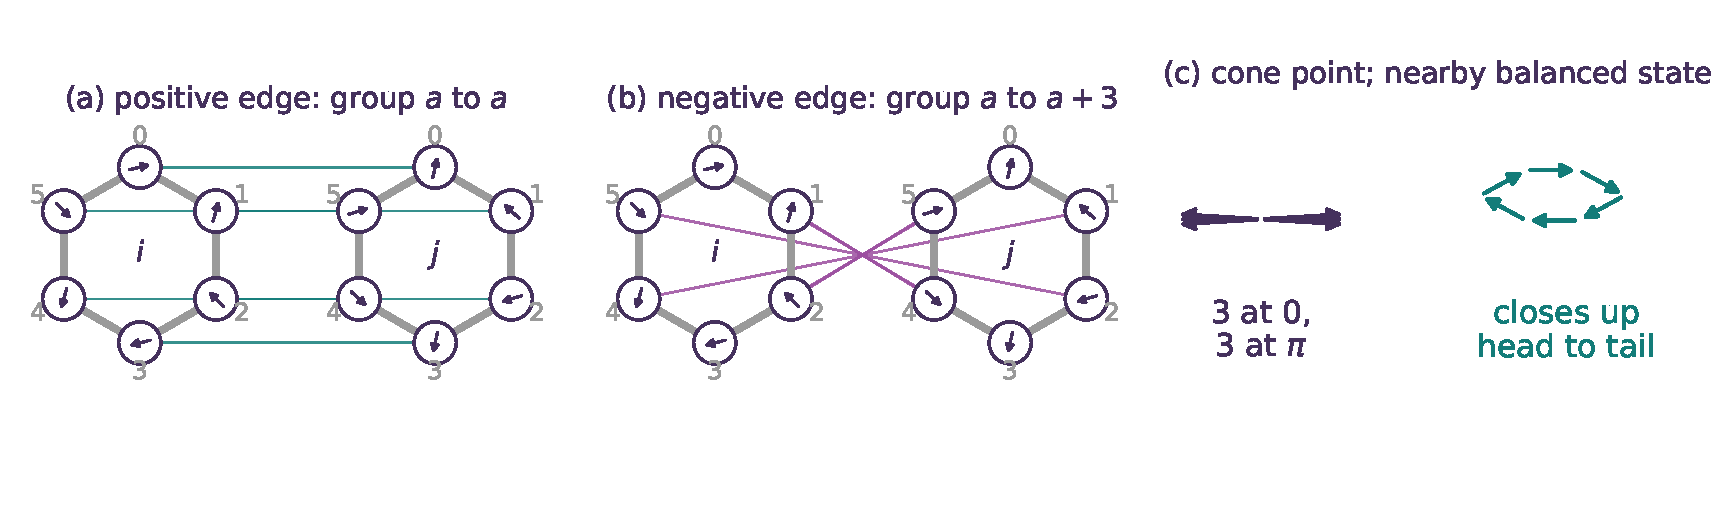
\includegraphics[width=\linewidth]{figures/kuramoto_construction.pdf}
\caption{The construction. (a,b) Each base vertex becomes a hexagonal ring of six groups. Grey ring edges join every clone in group $a$ to every clone in group $a\pm1$. Arrows show the phases $\phi_i+a\pi/3$ on the invariant torus. A positive base edge matches group $a$ of $i$ with group $a$ of $j$. A negative base edge matches group $a$ with group $a+3$, whose phase is shifted by $\pi$; this turns $+\sin$ into $-\sin$. (c) The cone point of $K_6$ and a nearby balanced state, drawn as a closed polygon.}\label{fig:construction}
\end{figure}

\section{The realisation theorem}\label{sec:realisation}

\subsection{Graph and invariant torus}
For a signed graph $H$ on $\{1,\dots,n\}$ and an integer $r\ge1$, set $V(G)=V(H)\times\Z_6\times\{1,\dots,r\}$. For each $i$ and $a\in\Z_6$ join every $(i,a,k)$ to every $(i,a+1,l)$. For each base edge $\{i,j\}$ put $d_{ij}=0$ if $\sigma_{ij}=1$ and $d_{ij}=3$ if $\sigma_{ij}=-1$, and add
\begin{equation}\label{eq:edges}
 (i,a,k)\sim(j,a+d_{ij},k),\qquad a\in\Z_6,\ 1\le k\le r.
\end{equation}
Because $d_{ij}=d_{ji}$ modulo~$6$, the rule is symmetric. The edges are distinct and there are no loops, which gives the counts in Theorem~\ref{thm:realisation}. Define
\begin{equation}\label{eq:embedding}
 F(\phi)_{i,a,k}=\phi_i+a\pi/3 .
\end{equation}
The map $F$ is affine on angle lifts, $F(\phi)=B\phi+c$, with $B^{\mathsf T}B=6rI_n$. It is injective modulo $2\pi$ because the $a=0$ coordinates recover $\phi$. Write $M=F(\T^n)$, $TM=\operatorname{ran}B$, and $N=TM^\perp$.

\emph{Invariance.} At $F(\phi)$ the ring neighbours of $(i,a,k)$ sit at offsets $\pm\pi/3$, so their sine contributions cancel. The cross neighbour across a base edge contributes $\sin(\phi_j-\phi_i+d_{ij}\pi/3)=\sigma_{ij}\sin(\phi_j-\phi_i)$, independently of $a$ and $k$. Hence the vector field of $G$ at $F(\phi)$ equals $B$ applied to the field~\eqref{eq:signed} at $\phi$. This holds at every point of $M$, not only at equilibria, so $M$ is invariant and carries~\eqref{eq:signed} exactly. Counting edges gives
\begin{equation}\label{eq:energyrestriction}
 E_G(F(\phi))=3nr^2+12re_-+6rE_H^\sigma(\phi),
\end{equation}
where $e_-$ is the number of negative edges. Each ring contributes $6r^2(1-\cos\frac\pi3)=3r^2$. A positive edge contributes $6r(1-\cos(\phi_j-\phi_i))$. A negative edge contributes $6r(1+\cos(\phi_j-\phi_i))=12r-6r(1-\cos(\phi_j-\phi_i))$.

\subsection{The normal Hessian}
Write $J(\theta)$ for the Jacobian of~\eqref{eq:flow}. It is symmetric, and $\nabla^2E_G=-J$. Split $J=J_{\rm int}+J_{\rm cross}$ by edge type. On $M$,
\[
 J_{\rm int}=\tfrac12 I_n\otimes A_6\otimes\mathbf J_r-rI,
\]
where $A_6$ is the adjacency matrix of the $6$-cycle and $\mathbf J_r$ the all-ones $r\times r$ matrix. On clone-constant vectors in ring Fourier mode $\ell$ its eigenvalue is $-r[1-\cos(\ell\pi/3)]$, and on clone vectors with sum zero it is $-r$. Its kernel is exactly $TM$ (the case $\ell=0$, clone-constant), and on $N$ it is $\preceq-\tfrac r2$. The cross part is $J_{\rm cross}=W-\operatorname{diag}(W\mathbf 1)$ with $|W_{uv}|\le1$ and at most $\Delta$ nonzero entries per row. Its row sums of absolute values are therefore at most $2\Delta$, and $\|J_{\rm cross}\|_2\le2\Delta$. For $z\in N$,
\begin{equation}\label{eq:normalbound}
 \langle z,\nabla^2E_G(F(\phi))z\rangle\ \ge\ \bigl(\tfrac r2-2\Delta\bigr)\|z\|^2\qquad\text{for all }\phi\in\T^n .
\end{equation}

\subsection{Normal coercivity and the energy inequality}
The next lemma holds at every point of $M$, including degenerate cone points. It is stated with a general constant $\mu$ so that the sharper bound of Section~\ref{sec:applications} can be used as well.

\begin{lemma}[Normal coercivity]\label{lem:coercive}
Let $\Omega\subset\R^n$ be open, and suppose $\langle z,\nabla^2E_G(F(\phi))z\rangle\ge\mu\|z\|^2$ for all $\phi\in\Omega$ and $z\in N$, with $\mu>0$. Let $D$ be the maximum degree of $G$, and put $\rho=\mu/(8D)$. Then for $\phi\in\Omega$ and $z\in N$ with $\|z\|<\rho$:
\begin{align}
 E_G(F(\phi)+z)&\ \ge\ E_G(F(\phi))+\tfrac{\mu}{4}\|z\|^2,\label{eq:energyinequality}\\
 \langle z,\nabla E_G(F(\phi)+z)\rangle&\ \ge\ \tfrac{\mu}{2}\|z\|^2.\label{eq:radial}
\end{align}
\end{lemma}
\begin{proof}
Put $g(\phi,z)=E_G(F(\phi)+z)$.

\emph{Step 1: $z=0$ is critical in the normal directions.} By invariance, $\nabla E_G(F(\phi))=-(\text{vector field at }F(\phi))\in TM$. Hence $\partial_zg(\phi,0)=P_N\nabla E_G(F(\phi))=0$ for every $\phi$, whether or not $\phi$ is an equilibrium.

\emph{Step 2: a Lipschitz bound for the Hessian.} We have $\nabla^2E_G(\theta)=L_{w(\theta)}$, the Laplacian with edge weights $w_{uv}=\cos(\theta_v-\theta_u)$. Since $|\cos s-\cos t|\le|s-t|$, each weight changes by at most $2\|\theta-\theta'\|_\infty$. A Laplacian has operator norm at most twice its largest absolute row sum of off-diagonal weights. Therefore
\[
 \|\nabla^2E_G(\theta)-\nabla^2E_G(\theta')\|_2\le4D\|\theta-\theta'\|.
\]

\emph{Step 3: Taylor's formula in $z$ with a remainder uniform in $\phi$.} Using Step~1,
\[
 g(\phi,z)-g(\phi,0)=\int_0^1(1-s)\,\langle z,\nabla^2E_G(F(\phi)+sz)z\rangle\,ds .
\]
By the hypothesis and Step~2, the integrand is at least $(\mu-4D\|z\|)\|z\|^2\ge\tfrac\mu2\|z\|^2$ when $\|z\|<\rho$. Integrating $(1-s)$ over $[0,1]$ gives the factor $\tfrac12$, which proves~\eqref{eq:energyinequality}. Similarly, $\langle z,\nabla E_G(F(\phi)+z)\rangle=\int_0^1\langle z,\nabla^2E_G(F(\phi)+sz)z\rangle ds\ge\tfrac\mu2\|z\|^2$, which proves~\eqref{eq:radial}.
\end{proof}

No nondegeneracy in the $\phi$ directions is assumed. At a cone vertex the tangential Hessian has extra zero eigenvalues, but~\eqref{eq:energyinequality} still holds with the same constants. ``Local minimum'' below always means non-strict: $x^\star$ is a local minimum of $f$ if $f\ge f(x^\star)$ on a neighbourhood. Such minima need not be isolated.

\subsection{Proof of Theorem~\ref{thm:realisation}}
Fix an equilibrium $\phi^\star$, lift it to $\R^n$, and let $\Omega$ be a ball around it. By~\eqref{eq:normalbound}, Lemma~\ref{lem:coercive} applies with $\mu=r/2-2\Delta>0$. Since $\R^{6nr}=TM\oplus N$ and $F$ is affine, the chart $(\phi,z)\mapsto F(\phi)+z$ is an affine bijection from $\Omega\times\{\|z\|<\rho\}$ onto a neighbourhood $\mathcal U$ of $F(\phi^\star)$.

(a) Let $F(\phi)+z\in\mathcal U$ be an equilibrium of $G$. Its gradient vanishes, so~\eqref{eq:radial} forces $z=0$. Thus every equilibrium in $\mathcal U$ lies on $M$. By the exact restricted dynamics, $F(\phi)$ is an equilibrium if and only if $\phi$ is. Hence $F$ maps the equilibria of $H$ in $\Omega$ bijectively onto the equilibria of $G$ in $\mathcal U$. No implicit-function argument is needed.

(b) If $\phi^\star$ is a local minimum of $E_H^\sigma$ on $\Omega'\subset\Omega$, then on the chart over $\Omega'$, by~\eqref{eq:energyinequality} and~\eqref{eq:energyrestriction},
\[
 E_G(F(\phi)+z)\ge E_G(F(\phi))=3nr^2+12re_-+6rE_H^\sigma(\phi)\ge E_G(F(\phi^\star)).
\]
Conversely, restricting to $z=0$ shows that a local minimum of $E_G$ at $F(\phi^\star)$ gives a local minimum of $E_H^\sigma$ at $\phi^\star$. Both energies are real analytic, and both flows are Euclidean negative gradient flows in local angle coordinates. Absil and Kurdyka~\cite{absil} (Theorem~3) prove that for a real-analytic function $f$, an equilibrium of $\dot x=-\nabla f(x)$ is Lyapunov stable if and only if it is a local minimum of $f$, whether or not the minimum is isolated. Lyapunov stability is local, so the theorem applies to the periodic lifts. Hence $F(\phi^\star)$ is stable if and only if $\phi^\star$ is. The same applies at every equilibrium in $\mathcal U$, all of which lie on $M$ by (a). So $F$ identifies the germs of the stable sets.

(c) This is Corollary~\ref{cor:spectral}.

\emph{Connectivity.} Each ring of $6r$ vertices is connected, because consecutive groups are completely joined. If $H$ is connected, every two rings are joined by a chain of matchings. \qed

\begin{corollary}[Spectral transfer]\label{cor:spectral}
At an equilibrium $\phi^\star$ of~\eqref{eq:signed}, with Jacobian $J_H(\phi^\star)$,
\[
 \operatorname{spec}J(F(\phi^\star))=\operatorname{spec}J_H(\phi^\star)\ \cup\ \operatorname{spec}\bigl(J(F(\phi^\star))|_N\bigr),
 \qquad J(F(\phi^\star))|_N\preceq-\bigl(\tfrac r2-2\Delta\bigr)I .
\]
In particular $F(\phi^\star)$ and $\phi^\star$ have the same Morse index and the same nullity.
\end{corollary}
\begin{proof}
Differentiating the invariance identity $X_G(F(\phi))=BX_H(\phi)$ gives $J(F(\phi))B=BJ_H(\phi)$. So $J$ maps $TM$ into itself, and by symmetry it also maps $N$ into itself. Since $B/\sqrt{6r}$ is an isometry onto $TM$, $J|_{TM}$ is orthogonally conjugate to $J_H$. The bound on $N$ is~\eqref{eq:normalbound}.
\end{proof}

\section{Balance geometry and the cover obstructions}\label{sec:topology}

\subsection{All local equilibrium branches}
Work with positive lengths $a_1,\dots,a_n$ and
\begin{equation}\label{eq:weighted}
 Z_a(\theta)=\sum_ja_je^{\ii\theta_j},\qquad B_a=Z_a^{-1}(0),\qquad
 \dot\theta_u=\pm a_u\sum_{v\neq u}a_v\sin(\theta_v-\theta_u).
\end{equation}
The sign $+$ gives the attractive rank-one network and $-$ the repulsive one; the two have the same equilibria. Let $\mathcal A_n$ be the aligned configurations, whose phases all lie in a pair $\{\alpha,\alpha+\pi\}$. Counting sign patterns up to a global flip, this is a disjoint union of $2^{n-1}$ phase circles.

\begin{lemma}\label{lem:branches}
The equilibrium set of~\eqref{eq:weighted} is $B_a\cup\mathcal A_n$. Near a balanced aligned point the whole equilibrium set agrees with $B_a$.
\end{lemma}
\begin{proof}
The $u$th component is $\pm a_u\im(Z_ae^{-\ii\theta_u})$. If $Z_a\neq0$, it vanishes for every $u$ exactly when each $e^{\ii\theta_u}$ is parallel or antiparallel to $Z_a$, that is, when the configuration is aligned. The aligned circles are finitely many and pairwise disjoint. A small neighbourhood of a balanced aligned point therefore meets only its own aligned circle, and that circle lies in $B_a$ because rotation preserves balance.
\end{proof}

\subsection{The local cone}
Suppose $\{1,\dots,n\}=P\sqcup Q$ with $p=|P|\ge2$, $q=|Q|\ge2$ and
\begin{equation}\label{eq:partition}
 \textstyle\sum_{i\in P}a_i=\sum_{j\in Q}a_j=A .
\end{equation}
Let $\theta^\star$ have phase $0$ on $P$ and $\pi$ on $Q$. In an angle chart write $\theta_i=\gamma+x_i$ for $i\in P$ and $\theta_j=\pi+\gamma+\delta+y_j$ for $j\in Q$, with $\sum_Pa_ix_i=\sum_Qa_jy_j=0$. This gives $1+1+(p-1)+(q-1)=n$ coordinates $(\gamma,\delta,x,y)$. Put $R_P=\sum_Pa_ie^{\ii x_i}$ and $R_Q=\sum_Qa_je^{\ii y_j}$. Both are close to $A>0$. Then $Z_a=e^{\ii\gamma}(R_P-e^{\ii\delta}R_Q)$, and $Z_a=0$ is equivalent to
\[
 |R_P(x)|=|R_Q(y)|\quad\text{and}\quad \delta=h(x,y):=\arg R_P(x)-\arg R_Q(y).
\]
Here $h$ is smooth near the origin. The deficits $D_P=A^2-|R_P|^2$ and $D_Q=A^2-|R_Q|^2$ satisfy
\begin{equation}\label{eq:deficit}
 D_P(x)=2\sum_{i<j\in P}a_ia_j[1-\cos(x_i-x_j)]=A\sum_{i\in P}a_ix_i^2+O(\|x\|^4)
\end{equation}
on the slice $\sum a_ix_i=0$, using $\sum_{i<j}a_ia_j(x_i-x_j)^2=A\sum a_ix_i^2-(\sum a_ix_i)^2$. So $D_P$ has a nondegenerate minimum $0$ at $x=0$ on the $(p-1)$-dimensional slice, and likewise for $D_Q$. The Morse lemma, applied separately in the disjoint variables $x$ and $y$, gives local diffeomorphisms $x\mapsto u\in\R^{p-1}$ and $y\mapsto v\in\R^{q-1}$ with $D_P=\|u\|^2$ and $D_Q=\|v\|^2$. Finally, $|R_P|=|R_Q|$ if and only if $D_P=D_Q$.

\begin{lemma}[The polygon cone in angle coordinates]\label{lem:cone}
Under~\eqref{eq:partition} there is a neighbourhood $W$ of $\theta^\star$ in the equilibrium set and a homeomorphism
\begin{equation}\label{eq:cone}
 W\ \cong\ \{(\gamma,u,v)\in I\times\R^{p-1}\times\R^{q-1}:\ \|u\|=\|v\|<\varepsilon\}\ \cong\ I\times C(S^{p-2}\times S^{q-2})
\end{equation}
taking $\theta^\star$ to $(0,\text{vertex})$, where $I$ is an open interval. The set
\begin{equation}\label{eq:regular}
 U=\{\|u\|=\|v\|>0\}\cong I\times(0,\varepsilon)\times S^{p-2}\times S^{q-2}
\end{equation}
is an open, dense smooth submanifold of $W$ of dimension $d=p+q-2$, and the singular set $W\setminus U=I\times\{\text{vertex}\}$ is an arc. If moreover $p,q\ge3$, then $U$ is connected, and for every smaller product neighbourhood $V$ of the vertex, $V\cap U$ is again connected and dense in $V$. If $p=q=2$, then $\{\|u\|=\|v\|\}=\{v=u\}\cup\{v=-u\}\subset\R^2$ is a pair of lines crossing at the origin, and $U$ has four components.
\end{lemma}
\begin{proof}
Here $W$ is the set of equilibria in a chart box $I\times\{|\delta|<\delta_0\}\times\{\|u\|,\|v\|<\varepsilon\}$, with $\varepsilon$ so small that $|h|<\delta_0$ on it, and $W$ is open in the equilibrium set because the box is open. By Lemma~\ref{lem:branches}, $W$ is the balanced set near $\theta^\star$. The coordinate change $(\gamma,\delta,x,y)\mapsto(\gamma,\delta,u,v)$ is a local diffeomorphism. In the new coordinates $W$ is the graph of the smooth function $\delta=h$ over the set $\{\|u\|=\|v\|\}$, and a graph is homeomorphic to its base. This gives the first homeomorphism. For the second, send $(\gamma,u,v)$ with $t=\|u\|=\|v\|>0$ to $(\gamma,[t,u/t,v/t])$, and send the points with $u=v=0$ to $(\gamma,\text{vertex})$. This map is a continuous bijection. Its inverse $(\gamma,[t,\xi,\eta])\mapsto(\gamma,t\xi,t\eta)$ is continuous, also at $t=0$, because $\|(t\xi,t\eta)\|=\sqrt2\,t$. Away from $u=v=0$, the function $\|u\|^2-\|v\|^2$ has nonzero gradient $(2u,-2v)$. Its zero set is therefore a smooth hypersurface of dimension $(p-1)+(q-1)-1$ in $(u,v)$-space, and with the $\gamma$ factor the dimension is $d$. The set $U$ is open because its complement $\{u=v=0\}$ is closed. It is dense because $(\gamma,0,0)=\lim_{t\to0}(\gamma,t\xi,t\eta)$. None of these steps uses $p,q\ge3$: for $p=q=2$ the Morse coordinates $u,v$ are real numbers and $\{|u|=|v|\}$ is the pair of lines $v=\pm u$, whose complement of the origin has four components, matching $C(S^0\times S^0)$. When $p,q\ge3$, $U$ is connected because $S^{p-2}$ and $S^{q-2}$ are connected. The same reasoning applies to $I'\times\{t<\varepsilon'\}$.
\end{proof}

This derivation is included to make the result checkable without importing a polygon-space convention. The cone itself is classical~\cite{kamiyama,kapovichmillson}. Burns et al.~\cite{burns}, Theorem~16.1, describe its tangent directions for $K_{2m}$.

\subsection{Local homology}
Let $L=S^{p-2}\times S^{q-2}$ and $o=(0,\text{vertex})\in\R\times C(L)$. The link of $o$ is the suspension $S^0*L=\Sigma L$, so
\begin{equation}\label{eq:homology}
 H_k\bigl(\R\times C(L),\ \R\times C(L)\setminus\{o\};\Z\bigr)\cong\widetilde H_{k-1}(\Sigma L)\cong\widetilde H_{k-2}(L).
\end{equation}
For $p,q\ge3$ these groups are nonzero exactly in degrees $p$, $q$ and $d=p+q-2$; the group in degree $p$ has rank two when $p=q$. A point of a $d$-manifold without boundary has local homology $\Z$ in degree $d$ only. Since $p<d$, the point $o$ has no neighbourhood that is a $d$-manifold. This is the only role homology plays below. The cover arguments use connectedness of the regular part.

\subsection{Countable closed covers}

\begin{lemma}[Closed-cover obstruction]\label{lem:cover}
Let $X$ be a Hausdorff space and $W\subset X$ an open set containing $o$. Let $U\subset W$ be open and dense in $W$, and suppose $U$ is a connected topological $d$-manifold. Suppose $W$ is not a $d$-manifold at $o$. Then $X$ is not a countable union of subsets $M_j$ that are closed in $X$ and are second-countable, finite-dimensional topological manifolds without boundary in the subspace topology.
\end{lemma}
\begin{proof}
Suppose $X=\bigcup_jM_j$. A second-countable manifold has countably many components, each closed in $M_j$ and hence in $X$. We may therefore assume that each $M_j$ is connected and has a single dimension $d_j$. The sets $M_j\cap U$ are closed in the locally compact Hausdorff space $U$ and cover it. By Baire's theorem some $O=\interior_U(M_j\cap U)$ is nonempty. Since $U$ is open in $X$, the set $O$ is open in $X$, hence open in $M_j$. A nonempty set that is open both in a $d$-manifold and in a $d_j$-manifold forces $d_j=d$, by invariance of dimension. By invariance of domain, $M_j\cap U$ is then an open subset of $U$: each of its points has a neighbourhood in $M_j$ homeomorphic to $\R^d$, sitting injectively inside the $d$-manifold $U$. So $M_j\cap U$ is nonempty, open and closed in the connected space $U$, and therefore $U\subset M_j$. Since $M_j$ is closed and $U$ is dense in $W$, we get $W\subset M_j$. Then $W$ is open in $M_j$, so $W$ is a $d$-manifold, which contradicts the hypothesis at $o$.
\end{proof}

The next lemma handles the branched reading. A topological immersion is a continuous map that is injective on a neighbourhood of each point.

\begin{lemma}[Immersed-cover obstruction]\label{lem:immersed}
Let $X,W,U,o,d$ be as in Lemma~\ref{lem:cover}. In addition, suppose that $o$ has arbitrarily small open neighbourhoods $V\subset W$ with $V\cap U$ connected and dense in $V$, and that $W\setminus U$ contains no subset homeomorphic to a nonempty open subset of $\R^d$. Then $X$ is not a countable union $\bigcup_jf_j(N_j)$, where each $N_j$ is a compact topological manifold without boundary and each $f_j:N_j\to X$ is a topological immersion.
\end{lemma}
\begin{proof}
A compact manifold has finitely many components, so we may assume each $N_j$ is connected, of dimension $d_j$. Each $K_j=f_j(N_j)$ is compact, hence closed in $X$.

\emph{Preliminary.} Let $f:N\to X$ be one of the immersions and let $y\in X$. The fibre $f^{-1}(y)$ is closed and discrete in the compact space $N$, so it is finite: $\{x_1,\dots,x_s\}$. Choose pairwise disjoint closed coordinate balls $\bar B_k$ centred at the $x_k$, so small that $f|_{\bar B_k}$ is injective and hence a homeomorphism onto its compact image. The set $f(N\setminus\bigcup_kB_k)$ is compact and does not contain $y$. The sets $f(\partial B_k)$ are compact and do not contain $y$ either. Hence every sufficiently small neighbourhood $V$ of $y$ satisfies
\begin{equation}\label{eq:sheets}
 V\cap f(N)=\bigcup_k V\cap f(B_k),\qquad V\cap f(\bar B_k)=V\cap f(B_k).
\end{equation}
If moreover $y\in U$, the balls can be chosen with $f(\bar B_k)\subset U$.

\emph{Step 1: the dimension.} As in Lemma~\ref{lem:cover}, Baire's theorem gives some $j$ with $O=\interior_U(K_j\cap U)\neq\emptyset$. Take $y\in O$ and apply the preliminary with a neighbourhood $V\subset O$ of $y$ that is open in $U$. Then $V$ is covered by the finitely many closed sets $V\cap f_j(\bar B_k)$. By Baire's theorem again, one of them contains a nonempty open subset $G$ of the $d$-manifold $V$. Since $V$ was chosen to avoid $f_j(\partial B_k)$, the open set $G\subset V\cap f_j(\bar B_k)$ lies in $f_j(B_k)$. The restriction $f_j|_{\bar B_k}$ is a homeomorphism onto its image, hence $f_j^{-1}(G)$ is a nonempty open subset of the $d_j$-manifold $B_k$ and is homeomorphic to $G$. Since $G$ is a nonempty open subset of the $d$-manifold $U$, invariance of dimension gives $d_j=d$.

\emph{Step 2: $W\subset K_j$.} Let $y\in K_j\cap U$, and take balls with $f_j(\bar B_k)\subset U$. Each $f_j(B_k)$ is the injective continuous image of an open $d$-ball in the $d$-manifold $U$, so it is open in $U$ by invariance of domain. By~\eqref{eq:sheets}, $y$ has a neighbourhood $V$ with $V\cap K_j$ equal to a union of open subsets of $U$. Thus $K_j\cap U$ is open in $U$. It is also closed in $U$ and nonempty, and $U$ is connected, so $U\subset K_j$. Since $K_j$ is closed and $U$ is dense in $W$, we get $W\subset K_j$; in particular $o\in K_j$.

\emph{Step 3: a single sheet covers a neighbourhood of $o$.} Apply the preliminary at $y=o$, and choose an open neighbourhood $V\subset W$ of $o$ that satisfies~\eqref{eq:sheets} and has $V\cap U$ connected and dense in $V$. Let $\Sigma_1=f_j(B_1)$; this is an embedded open $d$-ball containing $o$. The set $\Sigma_1\cap V$ is open in $\Sigma_1$ and nonempty. By hypothesis it is not contained in $W\setminus U$, so $\Sigma_1\cap V\cap U\neq\emptyset$. The set $\Sigma_1\cap V\cap U$ is open in $U$ by invariance of domain. By~\eqref{eq:sheets} it equals $f_j(\bar B_1)\cap V\cap U$, so it is closed in $V\cap U$. Connectedness gives $V\cap U\subset\Sigma_1$. Density of $V\cap U$ in $V$ and closedness of $f_j(\bar B_1)$ then give $V\subset f_j(\bar B_1)\cap V=\Sigma_1\cap V$. So $V\subset\Sigma_1$. Since $V$ is open in $X$, it is an open subset of the $d$-manifold $\Sigma_1$, and $W$ is a $d$-manifold at $o$. This is a contradiction.
\end{proof}

\begin{corollary}[Weighted obstruction]\label{cor:weighted}
Suppose a rank-one network~\eqref{eq:weighted} admits a partition~\eqref{eq:partition} with $p,q\ge3$. Then its equilibrium set $X$ is neither a countable union of closed embedded topological manifolds without boundary nor a countable union of immersed compact manifolds without boundary.
\end{corollary}
\begin{proof}
Lemma~\ref{lem:cone} supplies $W$, $U$, the small neighbourhoods $V$, and the arc $W\setminus U$. An arc contains no open subset of $\R^d$ with $d\ge4$. Equation~\eqref{eq:homology} shows that $W$ is not a $d$-manifold at $\theta^\star$. Now apply Lemmas~\ref{lem:cover} and~\ref{lem:immersed}.
\end{proof}

\section{Applications of the realisation theorem}\label{sec:applications}

\subsection{Repulsive complete graphs and a sharper constant}
Take $H=K_m$ with all signs negative, and write $G_{m,r}=G(K_m^-,r)$. The base flow is $\dot\phi=-\nabla\tfrac12|Z(\phi)|^2$ with $Z=\sum e^{\ii\phi_i}$. Its equilibria are the balanced and aligned configurations (Lemma~\ref{lem:branches}). Every balanced point is a global minimum. By~\eqref{eq:energyrestriction},
\begin{equation}\label{eq:specialenergy}
 E_{G_{m,r}}(F(\phi))=3mr^2+3rm(m-2)+3r|Z(\phi)|^2 .
\end{equation}
At a balanced point let $\Gamma_{ij}=\cos(\phi_j-\phi_i)$. This is a positive semidefinite Gram matrix with $\rank\Gamma\le2$, trace $m$, $\lambda_{\max}(\Gamma)\le m$ and $\Gamma\mathbf1=0$. Let $\Pi$ be the ring shift $a\mapsto a+3$. Then
\begin{equation}\label{eq:specialJ}
 J=\underbrace{\tfrac12 I_m\otimes A_6\otimes\mathbf J_r-rI}_{J_{\rm int}}+\underbrace{(I_m-\Gamma)\otimes\Pi\otimes I_r-I}_{J_{\rm cross}} .
\end{equation}
The diagonal of $J_{\rm cross}$ is $-1$ because $\sum_{j\ne i}\Gamma_{ij}=-1$ at a balanced point. On ring mode $\ell$, $\Pi$ acts as $(-1)^\ell$, which gives the blocks in Table~\ref{tab:blocks}.

\begin{table}[h]\centering\small
\caption{Jacobian blocks of $G_{m,r}$ at a balanced point.}\label{tab:blocks}
\begin{tabular}{lll}\toprule
Clone subspace & Ring mode & Block\\\midrule
constants & even $\ell$ & $-r[1-\cos(\ell\pi/3)]I_m-\Gamma$\\
constants & odd $\ell$ & $-r[1-\cos(\ell\pi/3)]I_m+\Gamma-2I_m$\\
sum zero & even $\ell$ & $-rI_m-\Gamma$\\
sum zero & odd $\ell$ & $-rI_m+\Gamma-2I_m$\\\bottomrule
\end{tabular}
\end{table}

\begin{proposition}\label{prop:sharper}
If $r>2(m-2)$, then at every balanced point $\phi^\star$ of $K_m$ the normal Hessian of $E_{G_{m,r}}$ is $\succeq(r/2-m+2)I$. Consequently conclusions (a) and (b) of Theorem~\ref{thm:realisation} hold at every balanced equilibrium of $K_m^-$ for $G_{m,r}$, on a neighbourhood of each balanced point, and conclusion (c) holds with the bound $-(r/2-m+2)$ in place of $-(r/2-2\Delta)$:
\[
 \operatorname{spec}J(F(\phi^\star))=\operatorname{spec}J_{K_m^-}(\phi^\star)\cup\operatorname{spec}\bigl(J|_N\bigr),\qquad J|_N\preceq-\bigl(\tfrac r2-m+2\bigr)I .
\]
In particular the Morse index and the nullity are preserved.
\end{proposition}
\begin{proof}
The tangent space is the clone-constant mode $\ell=0$, with block $-\Gamma$. Among the remaining blocks the largest eigenvalue is $-r/2+\lambda_{\max}(\Gamma)-2\le m-2-r/2$, attained in the clone-constant modes $\ell=1,5$. The normal Hessian is continuous in $\phi$, so it stays $\succeq\mu I$ with $\mu=\tfrac12(r/2-m+2)$ on a ball $\Omega$ around any balanced $\phi^\star$. Lemma~\ref{lem:coercive} applies on $\Omega$ with this $\mu$ and $D=2r+m-1$, so $\rho=\mu/(8D)$; the proofs of Theorem~\ref{thm:realisation}(a),(b) then go through unchanged. The spectral statement is the proof of Corollary~\ref{cor:spectral}, with the normal bound just computed in place of~\eqref{eq:normalbound}. The numerical bound $-(r/2-2\Delta)$ of Theorem~\ref{thm:realisation}(c) is not used, and need not be negative here: for $(m,r)=(6,9)$ it is $+\tfrac{11}2$.
\end{proof}

For $K_6$ this lowers the requirement from the general $r>4\Delta=20$, that is $r=21$, to $r=9$.

\begin{remark}[The threshold $r=9$ is sufficient, not shown to be sharp]\label{rem:threshold}
At the aligned balanced point $\theta^\star$ of $G_{6,r}$, the clone-constant modes $\ell=1,5$ on the $\Gamma$-eigenvector $s=(1,1,1,-1,-1,-1)$ have eigenvalue $4-r/2$. For $r\le7$ this is positive. Then $\theta^\star$ is not a local minimum: the energy decreases along that eigenvector to second order. So $\theta^\star$ is unstable, by Absil--Kurdyka or by Lyapunov's linear instability theorem. For $r=8$ the eigenvalue is $0$, the normal Hessian is degenerate at $\theta^\star$, and Lemma~\ref{lem:coercive} does not apply. We do not know whether $\theta^\star$ is stable for $r=8$. Hence $r=9$ is the smallest value for which our argument works, and $r>2(m-2)$ is a sufficient condition. The exact certificate confirms the eigenvalue $+\tfrac12$ (multiplicity two) at $r=7$ and the seven zero eigenvalues at $r=8$.
\end{remark}

\subsection{Proof of Theorem~\ref{thm:stable}}
Take $m=6$, $r=9$, $\phi^\star=(0,0,0,\pi,\pi,\pi)$ and $\theta^\star=F(\phi^\star)$. Then $G_{6,9}$ has $6mr=324$ vertices, degree $2r+m-1=23$, and $6mr^2+6r\binom m2=3726$ edges. It is connected because $K_6$ is. Near $\phi^\star$ the base equilibrium set is $B_6$, by Lemma~\ref{lem:branches}. By Proposition~\ref{prop:sharper} and part (a), there is a neighbourhood $O$ of $\theta^\star$ with $\E_G\cap O=F(B_6)\cap O$. Every point of $B_6$ is a global minimum of $|Z|^2$, hence stable, so by part (b) every point of $F(B_6)\cap O$ is stable. Therefore
\[
 \Sset_G\cap O=\E_G\cap O .
\]
Lemma~\ref{lem:cone} with $p=q=3$ gives the germ~\eqref{eq:stablecone}. The regular part has dimension $4$, and the local homology at $\theta^\star$ is $\Z^2$ in degree $3$ and $\Z$ in degree $4$. Apply Lemma~\ref{lem:cover} with $X=\E_G$ and with $X=\Sset_G$, taking $W=\E_G\cap O$ in both cases; this set is open in each $X$. Apply Lemma~\ref{lem:immersed}, again with $X=\E_G$ and with $X=\Sset_G$ and the same $W$; its extra hypotheses hold by Lemma~\ref{lem:cone} with $p=q=3$, and because the arc $W\setminus U$ contains no open subset of $\R^4$. No step of Lemma~\ref{lem:immersed} uses $X=\E_G$: for $X=\Sset_G$ the set $W=\Sset_G\cap O$ is open in $X$ and each image $f_j(N_j)$ is still compact. Lemma~\ref{lem:cover} needs only that the pieces are closed relative to $X$. This proves the theorem. \qed

At $\theta^\star$ the Jacobian has $5$ zero eigenvalues and $319$ negative ones (Section~\ref{sec:verification}). At nearby regular balanced points it has $4$ zero eigenvalues. A linearised test is therefore inconclusive at $\theta^\star$, and stability comes from the energy inequality~\eqref{eq:energyinequality}, not from the spectrum. In practice: when the Jacobian of a gradient system is singular, test local minimality of the energy. The neutral directions are genuine, and individual equilibria in the continuum are not asymptotically stable.

\subsection{Further applications}
\begin{corollary}[Stable cones of every even order]\label{cor:cones}
For every $m=2k+4\ge6$ and integer $r>2(m-2)$, the graph $G_{m,r}$ has a stable equilibrium continuum with germ $\R\times C(S^{k}\times S^{k})$ at $F(0^{m/2},\pi^{m/2})$. Neither its equilibrium set nor its stable set has a countable closed-manifold cover or a countable immersed compact cover.
\end{corollary}
\begin{proof}
This is the proof of Theorem~\ref{thm:stable} with $p=q=m/2=k+2\ge3$. Lemma~\ref{lem:cone} gives the link $S^{p-2}\times S^{q-2}=S^k\times S^k$ and a regular part of dimension $d=m-2\ge4$, so the singular arc contains no open subset of $\R^d$. For $m=6$ ($k=1$) this is the germ~\eqref{eq:stablecone}.
\end{proof}

\begin{corollary}[Stable crossing tori]\label{cor:crossing}
The graph $G_{4,5}$ (120 vertices, $13$-regular) has an open and closed subset of its equilibrium set, all of whose points are stable, that is the image of three embedded $2$-tori intersecting pairwise along aligned circles. At an aligned balanced point this set is locally two smooth surfaces intersecting cleanly along the common-phase circle, with distinct normal directions (they cross transversely inside the three-dimensional linearised balanced hypersurface, not in the ambient torus), and the Jacobian there has nullity $3$ rather than $2$. A finite closed cover exists here. So stability and a non-manifold point are compatible both with and without the cover obstruction; what decides the obstruction is the connectivity of the regular part near the singular point.
\end{corollary}
\begin{proof}
Use Proposition~\ref{prop:sharper} with $m=4$, $r=5$, together with the description $B_4=T_{12|34}\cup T_{13|24}\cup T_{14|23}$ given in Section~\ref{sec:classification}. Each pairing torus is compact. The three tori and their crossings are Sclosa's description of $B_4$~\cite{sclosa23}; what is new here is only their stable realisation in a positive unweighted graph. \emph{Open and closed.} For every $x\in F(B_4)$, Proposition~\ref{prop:sharper} and Theorem~\ref{thm:realisation}(a) give an ambient neighbourhood $O_x$ with $O_x\cap\E_{G_{4,5}}\subset F(\text{base equilibria})$. Since $B_4$ is closed in the base and at positive distance from the nonbalanced aligned circles, $O_x$ can be shrunk so that $O_x\cap\E_{G_{4,5}}\subset F(B_4)$. Hence $F(B_4)$ is open in $\E_{G_{4,5}}$. It is compact, as the continuous image of a compact set, and so closed in the Hausdorff space $\E_{G_{4,5}}$. By (b) its points are stable. \emph{Local picture.} At $(0,0,\pi,\pi)$, Lemma~\ref{lem:cone} with $p=q=2$, which holds in that range, gives $\{|u|=|v|\}=\{v=u\}\cup\{v=-u\}\subset\R^2$, two crossing lines; times the common-phase interval these are the two surfaces. Directly: only $T_{13|24}$ and $T_{14|23}$ pass through $(0,0,\pi,\pi)$, and their tangent planes $\{(a,b,a,b)\}$ and $\{(a,b,b,a)\}$ meet only in the diagonal direction, so the intersection is clean along the aligned circle. The nullity follows from Corollary~\ref{cor:spectral}: the base Jacobian there is $-\Gamma=-ss^{\mathsf T}$, which has nullity $3$.
\end{proof}

\begin{corollary}[Stable smooth continua of every dimension]\label{cor:smooth}
For odd $m\ge3$ and $r>2(m-2)$, the set $F(B_m)$ is a compact smooth $(m-2)$-dimensional manifold of stable equilibria of $G_{m,r}$. It is a union of components of $\E_{G_{m,r}}$, and the Jacobian has nullity exactly $m-2$ at each of its points.
\end{corollary}
\begin{proof}
For odd $m$, the set $B_m$ contains no aligned point and is a regular level set of $Z$, so it is a compact smooth $(m-2)$-manifold. At a balanced point the base Jacobian is $-\Gamma$, and $\rank\Gamma=2$, since the unit vectors are not all collinear when $m$ is odd. So its kernel has dimension $m-2=\dim B_m$, and Proposition~\ref{prop:sharper} gives nullity $m-2$ in $G_{m,r}$ and stability. \emph{Union of components.} For every $x\in F(B_m)$, Proposition~\ref{prop:sharper} and Theorem~\ref{thm:realisation}(a) give an ambient neighbourhood $O_x$ whose equilibria lie in $F$ of the base equilibria; as $B_m$ is at positive distance from the aligned circles, $O_x$ can be shrunk so that $O_x\cap\E_{G_{m,r}}\subset F(B_m)$. So $F(B_m)$ is open in $\E_{G_{m,r}}$. It is compact, hence closed in this Hausdorff space, and therefore a union of connected components.
\end{proof}
Sclosa~\cite{sclosa23} already constructs attractive networks with stable equilibrium manifolds of every dimension, and in doing so settles a conjecture of Delabays, Coletta and Jacquod~\cite{dcj} on the number of stable equilibria of connected planar graphs. Corollary~\ref{cor:smooth} is included because the realisation transfers the explicit polygon spaces $B_m$, and because it is certified at random balanced points for $m=5$.

\begin{remark}[A 36-vertex weighted version]\label{rem:weighted}
Replace the clone groups by single vertices ($r=1$) and give every ring edge weight $K$, keeping the unit antipodal cross matchings of $K_6^-$. The graph has six $6$-cycles and 36 vertices. All formulas above hold with the ring term $\tfrac K2 I_m\otimes A_6-KI$ in place of $J_{\rm int}$; clone deviations no longer occur. The ring mode $\ell$ contributes $-K[1-\cos(\ell\pi/3)]$, so the largest normal eigenvalue at a balanced point is $\le m-2-K/2=4-K/2$. For $K>8$ the normal Hessian is positive. \emph{Weighted coercivity.} Lemma~\ref{lem:coercive} extends to positive edge weights $\kappa_{uv}$ with $D$ replaced by $D_w=\max_u\sum_{v\sim u}\kappa_{uv}$: the Hessian is the Laplacian with weights $\kappa_{uv}\cos(\theta_v-\theta_u)$, each of which changes by at most $2\kappa_{uv}\|\theta-\theta'\|_\infty$, so Step~2 gives $\|\nabla^2E(\theta)-\nabla^2E(\theta')\|_2\le4D_w\|\theta-\theta'\|$, and Steps~1 and~3 are unchanged. Here $D_w=2K+5$, which is $23$ for $K=9$. The proof of Theorem~\ref{thm:stable} then applies word for word. For $K=9$ the computed spectrum at the cone point has largest normal eigenvalue $-\tfrac12$ and five zero eigenvalues. No minimal vertex count is claimed for either the weighted or the unweighted case.
\end{remark}

\section{The complete-graph classification}\label{sec:classification}

\begin{proof}[Proof of Theorem~\ref{thm:classification}]
Clearly (i)$\Rightarrow$(ii). A closed subset of the torus is compact, and an embedding of a compact manifold is an immersion; so (ii)$\Rightarrow$(iii). Next, (iii)$\Rightarrow$(iv): if $n=2m\ge6$, Corollary~\ref{cor:weighted} applies with unit lengths and $p=q=m$. It remains to show (iv)$\Rightarrow$(i).

For $n=1$ the equilibrium set is one circle, and for $n=2$ it is two aligned circles. For odd $n\ge3$, the derivative of $Z$ has rank $<2$ only at aligned configurations, and none of these is balanced because the two antipodal groups would need equal size. So $B_n$ is a compact smooth $(n-2)$-manifold, and $\E_n=B_n\cup\mathcal A_n$ is a finite union of closed manifolds.

For $n=4$, let $z_1,\dots,z_4$ be unit complex numbers with $\sum z_k=0$, and let $e_k$ be their elementary symmetric functions. For unit roots $\overline{e_k}=e_{4-k}/e_4$, so $e_3=e_4\overline{e_1}=0$, and $e_1=0$ as well. The polynomial $\prod(t-z_k)=t^4+e_2t^2+e_4$ is therefore even, and its roots, counted with multiplicity, are invariant under $t\mapsto-t$. Hence some labelled pairing satisfies $z_b=-z_a$ and $z_d=-z_c$. Writing
\[
 T_{12|34}=\{\theta_2=\theta_1+\pi,\ \theta_4=\theta_3+\pi\}\cong\T^2,
\]
and similarly $T_{13|24}$ and $T_{14|23}$, we get $B_4=T_{12|34}\cup T_{13|24}\cup T_{14|23}$. Adding the nonbalanced aligned circles, those with three phases equal or all four equal, gives a finite cover of $\E_4$ by closed embedded smooth manifolds.
\end{proof}

For $n=2m$, \eqref{eq:homology} reads $H_m=\Z^2$ and $H_{2m-2}=\Z$ at the cone point; for $K_6$ these are $H_3=\Z^2$ and $H_4=\Z$. We have not determined whether a smaller non-complete graph, for example $K_{3,3}$, which Sclosa analyses, already violates the closed reading. The minimality statement concerns complete graphs only.

\section{Verification}\label{sec:verification}

At $\theta^\star\in G_{6,9}$ we have $\Gamma=ss^{\mathsf T}$, with eigenvalues $6$ (once) and $0$ (five times). Table~\ref{tab:blocks} then gives the full spectrum:
\begin{center}\small
\begin{tabular}{rr@{\qquad}rr@{\qquad}rr}\toprule
Eigenvalue & Mult. & Eigenvalue & Mult. & Eigenvalue & Mult.\\\midrule
$-20$ & 5 & $-14$ & 1 & $-9$ & 120\\
$-19.5$ & 2 & $-13.5$ & 10 & $-6.5$ & 10\\
$-15$ & 24 & $-11$ & 120 & $-6$ & 1\\
$-5$ & 24 & $-0.5$ & 2 & $0$ & 5\\\bottomrule
\end{tabular}
\end{center}

The code is in the accompanying bundle. Python is pinned to version~3.12 and NumPy, SciPy and Matplotlib to exact versions; each script writes only to a directory given by \texttt{--out}.
\begin{itemize}
\item \texttt{verify\_attractive\_embedding.py} builds $G_{6,r}$ from the edge rule and verifies a complete integer tensor eigenbasis of $2J$ at $\theta^\star$, using exact integer arithmetic and no floating-point eigensolver. For $r=9$ it gives $319$ negative and $5$ zero eigenvalues. For $r=8$ it gives $7$ zero eigenvalues, and for $r=7$ the eigenvalue $+\tfrac12$ with multiplicity two (Remark~\ref{rem:threshold}).
\item \texttt{kuramoto\_checks.py} was written separately. (i) It checks the integer Kronecker identity~\eqref{eq:specialJ} and the first four trace powers of $2J$ exactly, and it checks invariance at random phases. The floating spectrum agrees with the exact list to within $10^{-12}$; the observed error, of order $10^{-14}$, depends on the platform's linear-algebra library. (ii) It checks Theorem~\ref{thm:realisation} on ten random connected signed graphs with $4$ to $7$ vertices, mixed signs and $r=4\Delta+1$. For each graph it checks the vertex, edge and degree counts, invariance, the energy identity~\eqref{eq:energyrestriction}, $J(TM)\subset TM$ and the normal bound~\eqref{eq:normalbound}. At 296 equilibria, namely all aligned states and the limits of gradient descent, with Morse indices $0$ to $5$ and nullities $1$ and $2$, it checks that the tangent spectrum equals the base spectrum to within $10^{-13}$ and that inertia is preserved (Corollary~\ref{cor:spectral}). (iii) For $G_{m,2m-3}$ with $m=4,5,6,8$ it checks zero force, the absence of positive eigenvalues, the normal bound of Proposition~\ref{prop:sharper}, and the predicted nullities. These are $3$ at the $K_4$ crossing, $3=m-2$ for $K_5$, $5$ and $7$ at the cone points of $K_6$ and $K_8$, and $m-2$ at nearby regular balanced points. (iv) It computes the 36-vertex weighted spectrum. (v) It samples the energy near $\theta^\star$ as numerical evidence of local minimality.
\item \texttt{reproduce.py} runs everything into a new output directory and compares the exact certificate and the edge list byte for byte with the shipped copies.
\end{itemize}
These checks corroborate the analytic proofs; they do not replace the topology or the nonlinear stability argument.

\section{Scope, robustness and prior work}\label{sec:prior}

\subsection{Scope and robustness}\label{sec:scope}
The singularities need equal-sum partitions~\eqref{eq:partition}. If the positive lengths admit no equal-sum partition of any sizes, so that no aligned configuration is balanced, then $B_a$ is a smooth manifold or empty. A partition with $p$ or $q\le2$ still produces a singular point, but not the connected-regular-part obstruction. The realisation is exact only for the specified graph and phase offsets. Small changes of weight or frequency need not preserve the invariant torus or the singularity. Individual equilibria in a continuum are not asymptotically stable. Real power grids, with heterogeneous injections and weighted lines, are outside the scope of these results.

\subsection{Identical-oscillator degeneracy}
Continua of equilibria of identical oscillators have a second, unrelated source. For globally coupled identical oscillators with sinusoidal coupling, Watanabe and Strogatz~\cite{ws} found $n-3$ constants of motion, which foliate phase space into invariant sets and produce neutral families. Ashwin and Swift~\cite{ashwinswift} classified the symmetry-forced cluster states of such systems. Ashwin, Burylko and Maistrenko~\cite{abm} found continua of neutrally stable equilibria in small Kuramoto--Sakaguchi networks. The cone here is different. It comes from the polygon geometry of balanced states, and in the lifted graph the reduction to $K_m$ is by an invariant torus, not by Watanabe--Strogatz variables. Stability of the continuum comes from the normal energy bound.

\subsection{Dense networks}
For identical oscillators with unit coupling, Taylor~\cite{taylor} proved that minimum degree at least $0.9395(n-1)$ excludes stable equilibria other than synchrony. Ling, Xu and Bandeira~\cite{lxb} lowered the constant to $0.7929$, and Kassabov, Strogatz and Townsend~\cite{kst} to $0.75$. Townsend, Stillman and Strogatz~\cite{tss} gave circulant networks of relative degree about $0.68$ with stable twisted states, which originate in the ring analysis of Wiley, Strogatz and Girvan~\cite{wsg}. The graph $G_{6,9}$ has relative degree $23/323\approx0.071$, and $G(H,r)$ has relative degree about $1/(3n)$ in general. These graphs are far below every density threshold, so there is no conflict: the results here concern the shape of stable sets in sparse graphs.

\subsection{Comparison table}
\begin{center}\small
\begin{tabular}{p{4.4cm}p{9.6cm}}\toprule
Known before & What is added here\\\midrule
Polygon cone at equal-sum lengths~\cite{kamiyama,kapovichmillson}; tangent link $S^{m-2}\times S^{m-2}$ for $K_{2m}$~\cite{burns} & Self-contained derivation of the local homeomorphism in Kuramoto angle coordinates (Lemma~\ref{lem:cone}); not claimed as new.\\
Balanced/aligned decomposition of $K_n$~\cite{hss,sclosa23} & Closed and immersed cover obstructions; classification (Theorem~\ref{thm:classification}).\\
Stable manifolds of equilibria of every dimension in attractive graphs~\cite{sclosa23} & Stable continua that are not manifolds (Theorem~\ref{thm:stable}, Corollaries~\ref{cor:cones}, \ref{cor:crossing}).\\
Weighted-to-unweighted lifts~\cite{canale}; quotient dynamics and signed equitable partitions~\cite{schaub}; coupled-cell synchrony and quotient networks~\cite{sgp,gst,gs} & Arbitrary signs by unit positive edges with phase offsets (the invariance step is of known type). New: the uniform normal bound, and, as its quantitative consequence, transfer of complete equilibrium germs, Lyapunov stability and spectra at degenerate equilibria (Lemma~\ref{lem:coercive}, Corollary~\ref{cor:spectral}, Theorem~\ref{thm:realisation}).\\\bottomrule
\end{tabular}
\end{center}

\paragraph{Priority against coupled-cell theory.} Stewart, Golubitsky and Pivato~\cite{sgp}, Golubitsky, Stewart and T\"or\"ok~\cite{gst}, and Golubitsky and Stewart~\cite{gs} show that balanced colourings give flow-invariant synchrony subspaces for every admissible vector field, and that the restricted dynamics is that of a quotient network. Their theory also describes phase patterns forced by network symmetry. Our torus $M$ is not a synchrony subspace, because the cells of a ring carry different phases. It is an invariant manifold of phase-shifted copies. Its invariance uses the $\Z_6$ symmetry of each ring together with the specific identity $\sin(x+\pi)=-\sin x$ of sine coupling. Its existence is of the same type as the invariance results of coupled-cell theory, and a reader familiar with that theory will regard the invariance step as expected. We have not found, in the works cited or in the Kuramoto literature we searched, a statement that realises arbitrary negative couplings by positive unit couplings while preserving complete equilibrium germs, nonlinear stability and spectra. The bounded search is described below. We checked~\cite{sgp,gst,gs} at the level of their main definitions and theorems, not exhaustively. The quantitative parts, namely the normal bound, Lemma~\ref{lem:coercive} and Corollary~\ref{cor:spectral}, are where we claim novelty; the transfer of germs, stability and spectra in Theorem~\ref{thm:realisation} is new only as a consequence of them. The invariance alone is not claimed as new. Phase-shift synchrony, graph coverings and voltage graphs, signed graph lifts and anti-phase quotients are the neighbouring literatures most likely to contain related statements.

\paragraph{Other comparisons.} Harrington, Schenck and Stillman~\cite{hss} (Example~2.12) give the complete-graph decomposition algebraically. Their notion of linear stability requires every non-phase eigenvalue to be strictly negative, so it does not cover the Lyapunov-stable degenerate states here. Chen, Korchevskaia and Lindberg~\cite{chen} study generic and nonisolated root counts. A non-manifold stable component like $F(B_6)$ produces singular witness points in a numerical irreducible decomposition, and might serve as a test case. Canale~\cite{canale} treats positive integer weights with a lift that preserves linearly stable equilibria; Schaub et al.~\cite{schaub} study cluster quotients with signed partitions. The literature search was current to 27 October 2026. It covered the originating papers, citing papers and searches under polygon linkage, balanced configuration, signed network, graph lift and equilibrium stratification. Absence from a bounded search does not establish priority.

\section*{Declarations}
\textbf{Authorship.} Anonymous. \textbf{AI provenance.} The mathematics, code and text were produced with substantial assistance from an AI system (Anthropic's Claude), working with a human research owner. The revision was guided by five simulated referee reports and an independent automated correctness review; a final round of corrections followed a targeted proof audit, a second automated correctness review and a fresh-context check of the corrected items. The proofs were checked by those AI-assisted reviews and by the computations described in Section~\ref{sec:verification}. The work has not been refereed externally and has not been formally verified in a proof assistant. \textbf{Code and data.} All scripts, the exact certificate, the edge list and the check outputs accompany this manuscript in the archive at \url{https://doi.org/10.5281/zenodo.23690073} and the repository \url{https://github.com/ipitchford/signed-kuramoto-positive-networks}; Section~\ref{sec:verification} gives the commands. \textbf{Licences.} Text CC0-1.0; code MIT. \textbf{Competing interests.} None. \textbf{Funding.} None.

\begin{thebibliography}{99}
\bibitem{absil} Absil, P.-A., \& Kurdyka, K. (2006). On the stable equilibrium points of gradient systems. \emph{Systems \& Control Letters, 55}(7), 573--577. \url{https://doi.org/10.1016/j.sysconle.2006.01.002}
\bibitem{abm} Ashwin, P., Burylko, O., \& Maistrenko, Y. (2008). Bifurcation to heteroclinic cycles and sensitivity in three and four coupled phase oscillators. \emph{Physica D, 237}(4), 454--466. \url{https://doi.org/10.1016/j.physd.2007.09.015}
\bibitem{ashwinswift} Ashwin, P., \& Swift, J. W. (1992). The dynamics of $n$ weakly coupled identical oscillators. \emph{Journal of Nonlinear Science, 2}(1), 69--108. \url{https://doi.org/10.1007/BF02429852}
\bibitem{bcr} Bochnak, J., Coste, M., \& Roy, M.-F. (1998). \emph{Real Algebraic Geometry}. Springer. \url{https://doi.org/10.1007/978-3-662-03718-8}
\bibitem{burns} Burns, D., Malajovich, G., Pugh, C., Rajapakse, I., \& Smale, S. (2026). \emph{Global analysis of the Kuramoto flow}. arXiv:2605.22983v3 (Section~16, Theorem~16.1). \url{https://arxiv.org/abs/2605.22983v3}
\bibitem{canale} Canale, E. A. (2022). \emph{From weighted to unweighted graphs in Synchronizing Graph Theory}. arXiv:2209.06362v3. \url{https://arxiv.org/abs/2209.06362}
\bibitem{chen} Chen, T., Korchevskaia, E., \& Lindberg, J. (2026). On the typical and atypical solutions to the Kuramoto equations. \emph{SIAM Journal on Applied Algebra and Geometry, 10}(2), 412--449. \url{https://doi.org/10.1137/24M1696718}
\bibitem{dcj} Delabays, R., Coletta, T., \& Jacquod, P. (2017). Multistability of phase-locking in equal-frequency Kuramoto models on planar graphs. \emph{Journal of Mathematical Physics, 58}(3), 032703. \url{https://doi.org/10.1063/1.4978697}
\bibitem{gs} Golubitsky, M., \& Stewart, I. (2006). Nonlinear dynamics of networks: the groupoid formalism. \emph{Bulletin of the American Mathematical Society, 43}(3), 305--365. \url{https://doi.org/10.1090/S0273-0979-06-01108-6}
\bibitem{gst} Golubitsky, M., Stewart, I., \& T\"or\"ok, A. (2005). Patterns of synchrony in coupled cell networks with multiple arrows. \emph{SIAM Journal on Applied Dynamical Systems, 4}(1), 78--100. \url{https://doi.org/10.1137/040612634}
\bibitem{hss} Harrington, H., Schenck, H., \& Stillman, M. (2025; issue 2026). Algebraic aspects of homogeneous Kuramoto oscillators. \emph{Mathematics of Computation, 95}(358), 1023--1047. Published online 18 February 2025. \url{https://doi.org/10.1090/mcom/4072}
\bibitem{kamiyama} Kamiyama, Y. (1996). Topology of equilateral polygon linkages. \emph{Topology and its Applications, 68}(1), 13--31. \url{https://doi.org/10.1016/0166-8641(96)00046-6}
\bibitem{kapovichmillson} Kapovich, M., \& Millson, J. J. (1996). The symplectic geometry of polygons in Euclidean space. \emph{Journal of Differential Geometry, 44}(3), 479--513. \url{https://doi.org/10.4310/jdg/1214459218}
\bibitem{kst} Kassabov, M., Strogatz, S. H., \& Townsend, A. (2021). Sufficiently dense Kuramoto networks are globally synchronizing. \emph{Chaos, 31}(7), 073135. arXiv:2105.11406. \url{https://doi.org/10.1063/5.0057659}
\bibitem{lxb} Ling, S., Xu, R., \& Bandeira, A. S. (2019). On the landscape of synchronization networks: A perspective from nonconvex optimization. \emph{SIAM Journal on Optimization, 29}(3), 1879--1907. arXiv:1809.11083. \url{https://doi.org/10.1137/18M1217644}
\bibitem{schaub} Schaub, M. T., O'Clery, N., Billeh, Y. N., Delvenne, J.-C., Lambiotte, R., \& Barahona, M. (2016). Graph partitions and cluster synchronization in networks of oscillators. \emph{Chaos, 26}(9), 094821. \url{https://doi.org/10.1063/1.4961065}
\bibitem{sclosa23} Sclosa, D. (2023). Kuramoto networks with infinitely many stable equilibria. \emph{SIAM Journal on Applied Dynamical Systems, 22}(4), 3267--3283. arXiv:2207.08182. \url{https://doi.org/10.1137/23M155400X}
\bibitem{sclosa25} Sclosa, D. (2025; online 2024). From combinatorics to geometry: The dynamics of graph gradient diffusion. \emph{Geometriae Dedicata, 219}(1), Article 6. arXiv:2308.08311. \url{https://doi.org/10.1007/s10711-024-00967-3}
\bibitem{sgp} Stewart, I., Golubitsky, M., \& Pivato, M. (2003). Symmetry groupoids and patterns of synchrony in coupled cell networks. \emph{SIAM Journal on Applied Dynamical Systems, 2}(4), 609--646. \url{https://doi.org/10.1137/S1111111103419896}
\bibitem{taylor} Taylor, R. (2012). There is no non-zero stable fixed point for dense networks in the homogeneous Kuramoto model. \emph{Journal of Physics A: Mathematical and Theoretical, 45}(5), 055102. arXiv:1109.4451. \url{https://doi.org/10.1088/1751-8113/45/5/055102}
\bibitem{tss} Townsend, A., Stillman, M., \& Strogatz, S. H. (2020). Dense networks that do not synchronize and sparse ones that do. \emph{Chaos, 30}(8), 083142. arXiv:1906.10627. \url{https://doi.org/10.1063/5.0018322}
\bibitem{ws} Watanabe, S., \& Strogatz, S. H. (1994). Constants of motion for superconducting Josephson arrays. \emph{Physica D, 74}(3--4), 197--253. \url{https://doi.org/10.1016/0167-2789(94)90196-1}
\bibitem{wsg} Wiley, D. A., Strogatz, S. H., \& Girvan, M. (2006). The size of the sync basin. \emph{Chaos, 16}(1), 015103. \url{https://doi.org/10.1063/1.2165594}
\end{thebibliography}
\end{document}
